\documentclass[11pt]{article}
\usepackage{enumitem}
\usepackage{listings}
\usepackage{tikz}
\usepackage{url}
%\usepackage{algorithm2e}
\usetikzlibrary{arrows,automata,shapes}
\tikzstyle{block} = [rectangle, draw, fill=blue!20, 
    text width=5em, text centered, rounded corners, minimum height=2em]
\tikzstyle{bt} = [rectangle, draw, fill=blue!20, 
    text width=4em, text centered, rounded corners, minimum height=2em]

\lstset{ %
language=Java,
basicstyle=\ttfamily,commentstyle=\scriptsize\itshape,showstringspaces=false,breaklines=true,numbers=left}

\newtheorem{defn}{Definition}
\newtheorem{crit}{Criterion}

\newcommand{\handout}[5]{
  \noindent
  \begin{center}
  \framebox{
    \vbox{
      \hbox to 5.78in { {\bf Software Testing, Quality Assurance and Maintenance } \hfill #2 }
      \vspace{4mm}
      \hbox to 5.78in { {\Large \hfill #5  \hfill} }
      \vspace{2mm}
      \hbox to 5.78in { {\em #3 \hfill #4} }
    }
  }
  \end{center}
  \vspace*{4mm}
}

\newcommand{\lecture}[4]{\handout{#1}{#2}{#3}{#4}{Lecture #1}}
\topmargin 0pt
\advance \topmargin by -\headheight
\advance \topmargin by -\headsep
\textheight 8.9in
\oddsidemargin 0pt
\evensidemargin \oddsidemargin
\marginparwidth 0.5in
\textwidth 6.5in

\parindent 0in
\parskip 1.5ex
%\renewcommand{\baselinestretch}{1.25}

\usepackage{fontspec}
\setmonofont{Cousine}[Scale=MatchLowercase]

\begin{document}

\lecture{8 --- January 20, 2017}{Winter 2017}{Patrick Lam}{version 1}

\paragraph{Larger CFG example.} You can draw a 7-node CFG for this program:

\begin{lstlisting}[basicstyle=\scriptsize\ttfamily]
  /** Binary search for target in sorted subarray a[low..high] */
  int binary_search(int[] a, int low, int high, int target) {
    while (low <= high) {
      int middle = low + (high-low)/2;
      if (target < a[middle)
        high = middle - 1;
      else if (target > a[middle])
        low = middle + 1;
      else
        return middle;
    }
    return -1; /* not found in a[low..high] */
  }
\end{lstlisting}

\vspace*{-2em}
\begin{center}
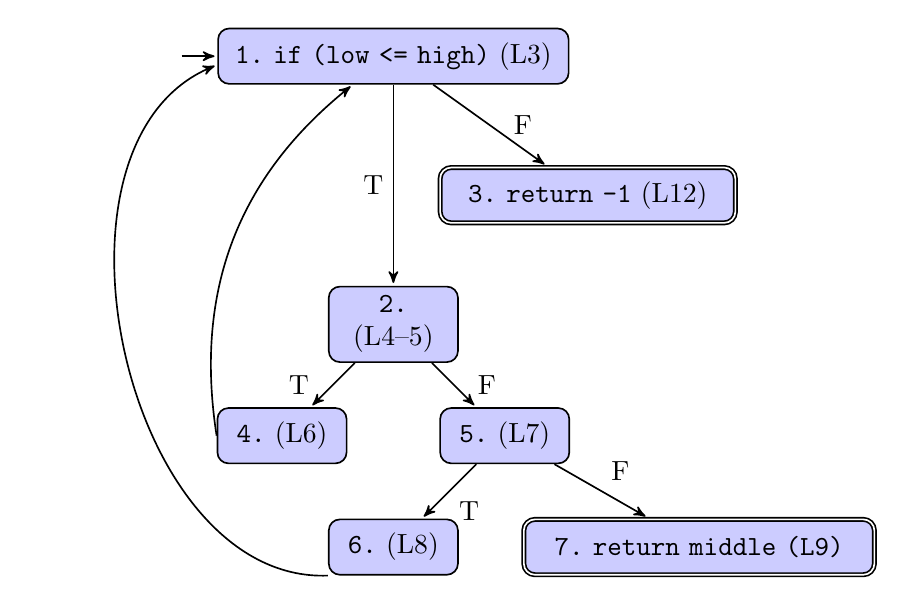
\begin{tikzpicture}[->,>=stealth',shorten >=1pt,auto,node distance=2cm,
                    semithick,initial text=]
  \node[initial,bt,text width=12em]   (1)                     {\verb+1. if (low <= high)+ (L3)};
  \node[bt, accepting,text width=10em]          (8) [below right of=1,yshift=-1em,xshift=3em]  {\verb+3. return -1+ (L12)};
  \node[bt]           (2) [below of=1, yshift=-4em]  {\verb+2.+ (L4--5)};
  \node[bt]           (4) [below left of=2] {\verb+4.+ (L6)};
  \node[bt]           (5) [below right of=2] {\verb+5.+ (L7)};
  \node[bt]           (6) [below left of=5] {\verb+6.+ (L8)};
  \node[bt,text width=12em,accepting,xshift=3em]           (7) [below right of=5] {\verb+7. return middle (L9)+};

  \path (1) edge node[left] {T} (2)
  (1) edge node[right,xshift=.5em] {F} (8)
  (2) edge node[left,xshift=-.5em] {T} (4)
  (2) edge node[right,xshift=.5em]{F} (5)
  (4.west) edge [bend left] (1)
  (5) edge node {T} (6)
  (5) edge node {F} (7)
  (6.south west) edge [bend left=80] (1);
\end{tikzpicture}
\end{center}

Here are more exercise programs that you can draw CFGs for.
\begin{lstlisting}[basicstyle=\scriptsize\ttfamily]
/* effects: if x==null, throw NullPointerException
            otherwise, return number of elements in x that are odd, positive or both. */
int oddOrPos(int[] x) {
  int count = 0;
  for (int i = 0; i < x.length; i++) {
    if (x[i]%2 == 1 || x[i] > 0) {
      count++;
    }
  }
  return count;
}

// example test case: input: x=[-3, -2, 0, 1, 4]; output: 3  
\end{lstlisting}

\newpage
Finally, we have a really poorly-designed API (I'd give it a D at most,
maybe an F) because it's impossible to succinctly describe what it
does. {\bf Do not design functions with interfaces like this.} But we
can still draw a CFG, no matter how bad the code is.
\begin{lstlisting}[basicstyle=\scriptsize\ttfamily]
  /** Returns the mean of the first maxSize numbers in the array,
      if they are between min and max. Otherwise, skip the numbers. */
  double computeMean(int[] value, int maxSize, int min, int max) {
    int i, ti, tv, sum;

    i = 0; ti = 0; tv = 0; sum = 0;
    while (ti < maxSize) {
      ti++;
      if (value[i] >= min && value[i] <= max) {
        tv++;
        sum += value[i];
      }
      i++;
    }
    if (tv > 0)
      return (double)sum/tv;
    else
      throw new IllegalArgumentException();
  }
\end{lstlisting}

\subsection*{Statement and Branch Coverage}
We defined Control-Flow Graphs so that we can give principled definitions of
statement and branch coverage. We can start with the definition of a test path:

\begin{defn} A \emph{test path} is a path $p$ (possibly of length 0)
that starts at some initial node (i.e. in $N_0$) and ends at some final node (i.e. in $N_f$).
\end{defn}

Here's a definition of coverage for graphs:
\begin{defn}
Given a set of test requirements \emph{TR} for a graph criterion $C$, 
a test set $T$ satisfies $C$ on graph $G$ iff for every test requirement
\emph{tr} in \emph{TR}, at least one test path $p$ in $\mbox{path}(T)$ 
exists such that $p$ satisfies \emph{tr}.
\end{defn}
We'll use this notion to define a number of standard testing
coverage criteria. But first, what are test paths?

\paragraph{Test cases and test paths.} We connect test cases and
test paths with a mapping $\mbox{path}_G$ from test cases to test
paths; e.g. $\mbox{path}_G(t)$ is the set of test paths corresponding
to test case $t$.
\begin{itemize}
\item usually we just write $\mbox{path}$ since $G$ is obvious from the context.
\item we can lift the definition of $\mbox{path}$ to test sets $T$ by defining
$\mbox{path}(T) = \{ \mbox{path}(t) | t \in T \}$.
\item each test case gives at least one test path. If the software is
  deterministic, then each test case gives exactly one test path;
  otherwise, multiple test cases may arise from one test path.
\end{itemize}

\newpage
\paragraph{Example.} Here is a short method, the associated control-flow
graph, and some test cases and test paths.

\begin{center}
\begin{minipage}{10em}
\vspace*{-8em}
\begin{lstlisting}
int foo(int x) {
  if (x < 5) {
    x ++;
  } else {
    x --;
  }
  return x;
}
\end{lstlisting}
\end{minipage}
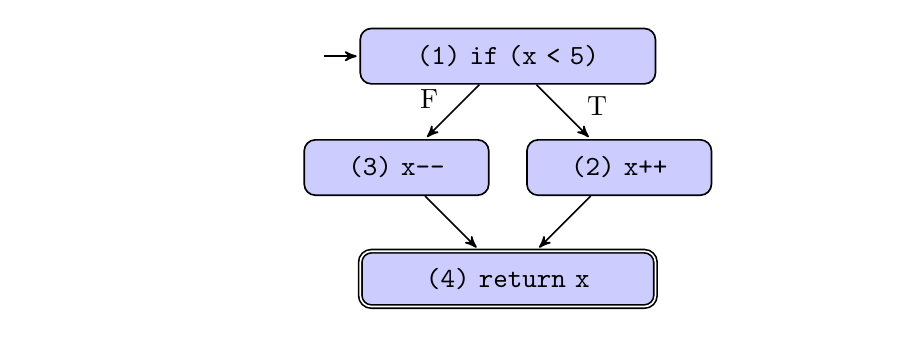
\begin{tikzpicture}[->,>=stealth',shorten >=1pt,auto,node distance=2cm,
                    semithick,text width=10em,initial text=]

  \node[initial,block,text width=10em]   (A)              {\tt (1) if (x < 5)};
  \node[block,text width=6em]           (T) [below right of=A] {\tt (2) x++};
  \node[block,text width=6em]           (F) [below left of=A] {\tt (3) x--};
  \node[accepting,block,text width=10em] (C) [below left of=T] {\tt (4) return x};

  \draw (A) -> (T) node [near end] {T};
  \draw (A) -> (F) node [yshift=.2em, xshift=-2.5em,at start] {F};
  \draw (T) -> (C);
  \draw (F) -> (C);
\end{tikzpicture}
\end{center}

\begin{itemize}
\item Test case: $x = 5$; test path: $[(1), (3), (4)]$.
\item Test case: $x = 2$; test path: $[(1), (2), (4)]$.
\end{itemize}

Note that (1) we can deduce properties of the test case from the test path; and
(2) in this example, since our method is deterministic, the test case 
determines the test path.

\paragraph{Nondeterminism.}
I mentioned the mapping between test cases and test paths above.
The mapping is not one-to-one for nondeterminstic code.
Here's an example of deterministic and nondeterministic control-flow graphs:
\begin{center}
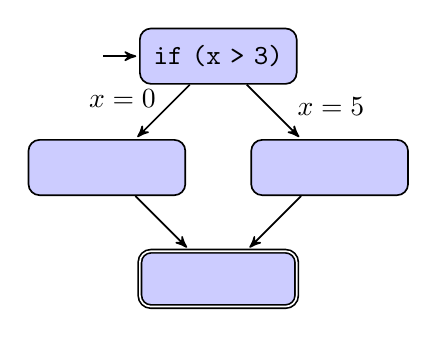
\begin{tikzpicture}[->,>=stealth',shorten >=1pt,auto,node distance=2cm,
                    semithick,initial text=]

  \node[initial,block,text width=5em]   (A)              {\tt if (x > 3)};
  \node[block]           (T) [below right of=A] {};
  \node[block]           (F) [below left of=A] {};
  \node[accepting,block] (C) [below left of=T] {};
  
  \draw (A) -> (T) node [near end] {$x = 5$};
  \draw (A) -> (F) node [yshift=.2em, xshift=-4em,at start] {$x = 0$};
  \draw (T) -> (C);
  \draw (F) -> (C);

\end{tikzpicture}
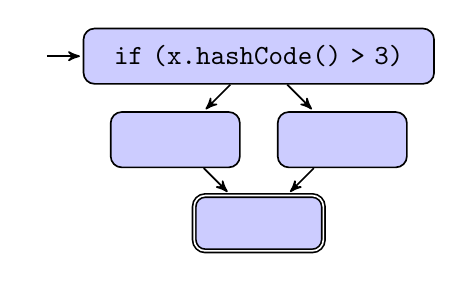
\begin{tikzpicture}[->,>=stealth',shorten >=1pt,auto,node distance=1.5cm,
                    semithick,initial text=]

  \node[initial,block,text width=12em]   (A)              {\tt if (x.hashCode() > 3)};
  \node[bt]           (T) [below right of=A] {};
  \node[bt]           (F) [below left of=A] {};
  \node[accepting,bt] (C) [below left of=T] {};
  
  \path (A) edge              node {} (T)
        (A) edge              node {} (F)
        (T) edge              node {} (C)
        (F) edge              node {} (C);
\end{tikzpicture}
\end{center}
Causes of nondeterminism include dependence on inputs; on the thread
scheduler; and on memory addresses, for instance as seen in calls to 
the default Java {\tt hashCode()} implementation. 

Nondeterminism makes it hard to check test case output, since more
than one output might be a valid result of a single test input.

\newpage
As another (more abstract) example, consider the double-diamond graph $D$.
\begin{center}
\label{D}
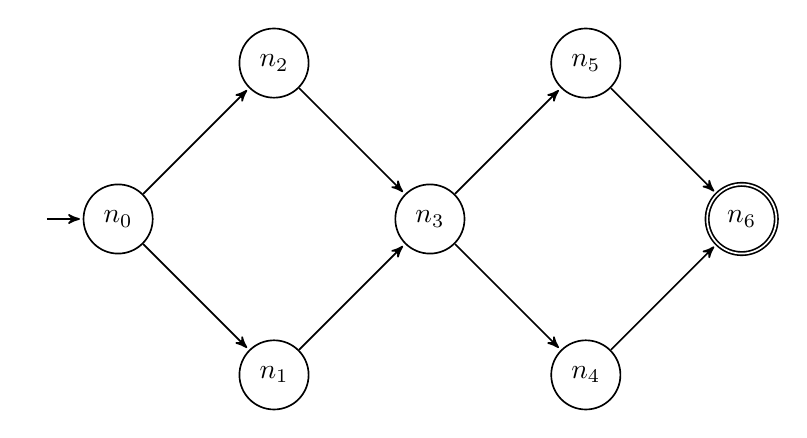
\begin{tikzpicture}[->,>=stealth',shorten >=1pt,auto,node distance=2.8cm,
                    semithick,initial text=]

  \node[initial,state]   (n0)                     {$n_0$};
  \node[state]           (n1) [below right of=n0] {$n_1$};
  \node[state]           (n2) [above right of=n0] {$n_2$};
  \node[state]           (n3) [below right of=n2] {$n_3$};
  \node[state]           (n4) [below right of=n3] {$n_4$};
  \node[state]           (n5) [above right of=n3] {$n_5$};
  \node[accepting,state] (n6) [below right of=n5] {$n_6$};
  
  \path (n0) edge              node {} (n1)
             edge              node {} (n2)
        (n1) edge              node {} (n3)
        (n2) edge              node {} (n3)
        (n3) edge              node {} (n4)
        (n3) edge              node {} (n5)
        (n4) edge              node {} (n6)
        (n5) edge              node {} (n6);
\end{tikzpicture}
\end{center}
Here are the four test paths in $D$:
\begin{eqnarray*}
&[n_0, n_1, n_3, n_4, n_6]& \\
&[n_0, n_1, n_3, n_5, n_6]& \\
&[n_0, n_2, n_3, n_4, n_6]& \\
&[n_0, n_2, n_3, n_5, n_6]&
\end{eqnarray*}

For the \emph{statement coverage} criterion, we get the following test requirements:
\[ \{ n_0, n_1, n_2, n_3, n_4, n_5, n_6 \} \]
That is, any test set $T$ which satisfies statement coverage on $D$ must include
test cases $t$; the cases $t$ give rise to test paths $\mbox{path}(t)$, and
some path must include each node from $n_0$ to $n_6$. (No single path must
include all of these nodes; the requirement applies to the set of
test paths.)

Let's formally define statement coverage.
\begin{defn}
Statement coverage: For each node $n \in \mbox{reach}_G(N_0)$, \emph{TR} contains
a requirement to visit node $n$.
\end{defn}

For our example,
\[ \mathit{TR} = \{ n_0, n_1, n_2, n_3, n_4, n_5, n_6\}. \]

Let's consider an example of a test set which satisfies statement coverage
on $D$.

Start with a test case $t_1$; assume that executing $t_1$ gives the
test path 
\[ \mbox{path}(t_1) = p_1 = [n_0, n_1, n_3, n_4, n_6].\] 
Then
test set $\{ t_1\}$ does not give statement coverage on $D$, because no
test case covers node $n_2$ or $n_5$. If we can find a test case $t_2$
with test path 
\[\mbox{path}(t_2) = p_2 = [n_0, n_2, n_3, n_5, n_6],\]
then the test set $T = \{ t_1, t_2 \}$ satisfies statement coverage on $D$.

{\sf What is another test set which satisfies statement coverage on $D$?}\\[2em]

%We could also satisfy node coverage with test set $T'$ containing test
%cases $t_1$ and new cases $t_3$ and $t_4$ where $p_3 = [n_0, n_2, n_3,
%n_4, n_6]$ and $p_4 = [n_0, n_1, n_3, n_5, n_6]$.

Here is a more verbose definition of statement coverage.

\begin{defn}
Test set $T$ satisfies \emph{statement coverage} on graph $G$ if and only
if for every syntactically reachable node $n \in N$, there is some
path $p$ in $\mbox{path}(T)$ such that $p$ visits $n$.
\end{defn}

A second standard criterion is that of branch coverage.
\begin{crit}
{\bf Branch Coverage}. TR contains each reachable path of length up
to 1, inclusive, in $G$.
\end{crit}

{\sf Here are some examples of paths of length $\le 1$:}\\[1em]
%\[ [n_3]; \qquad [n_4, n_6]. \]
Note that since we're not talking about \emph{test paths}, these
reachable paths need not start in $N_0$.

In general, paths of length $\le 1$ consist of nodes and edges. {\sf (Why not just
say edges?)}\\[3em]

%Consider this graph:
%\begin{center}
%\begin{tikzpicture}...
%\node[state,initial,accepting] (A) {};
%\end{tikzpicture}
%\end{center}
Saying ``edges'' on the above graph would not be the same as saying ``paths
of length $\le 1$''.

\paragraph{Another example.} Here is a more involved example:

\tikzstyle{block} = [rectangle, draw, fill=blue!20, 
    text width=3em, text centered, rounded corners, minimum height=2em]

\begin{center}
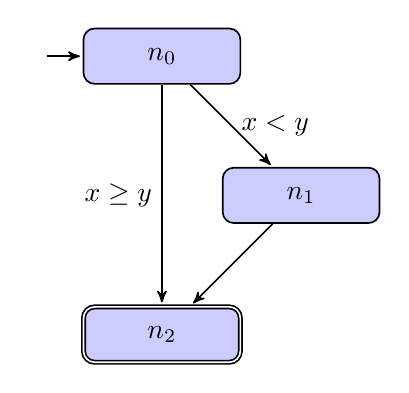
\begin{tikzpicture}[->,>=stealth',shorten >=1pt,auto,node distance=2.5cm,
                    semithick,initial text=]

  \node[initial,block]   (A)              {$n_0$};
  \node[block]           (B) [below right of=A] {$n_1$};
  \node[accepting,block] (C) [below left of=B] {$n_2$};
  
  \path (A) edge              node[right] {$x < y$} (B)
        (A) edge              node[left] {$x \ge y$} (C)
        (B) edge              node {} (C);
\end{tikzpicture}
\end{center}

Let's define
\begin{eqnarray*}
\mbox{path}(t_1) &=& [n_0, n_1, n_2] \\
\mbox{path}(t_2) &=& [n_0, n_2] 
\end{eqnarray*}

Then 
\begin{eqnarray*}
T_1 &=& \langle ? \rangle \hspace*{5em} \mbox{\sf satisfies statement coverage}\\
T_2 &=& \langle ? \rangle \hspace*{5em} \mbox{\sf satisfies branch coverage}
\end{eqnarray*}



\end{document}
